%%%%%%%%%%%%%%%%%%%%%%%%%%%%%%%%%%%%%%%%%%%%%%%%%%%%%%%%
%%%%%%%%%%%%%%%%%%%%%%%%%%%%%%%%%%%%%%%%%%%%%%%%%%%%%%%%
%%%                                                  %%%
%%% University of Arizona themed Beamer presentation %%%
%%% Based on the Warsaw, Palo Alto and UNL templates %%%
%%% modified by Joseph V. Casillas (6-13-2011)       %%%
%%%                                                  %%%
%%%%%%%%%%%%%%%%%%%%%%%%%%%%%%%%%%%%%%%%%%%%%%%%%%%%%%%%
%%%%%%%%%%%%%%%%%%%%%%%%%%%%%%%%%%%%%%%%%%%%%%%%%%%%%%%%

\documentclass{beamer}
\mode<presentation>{\usetheme{Madrid}\setbeamercovered{transparent}}
\usepackage[english]{babel}
\usepackage[utf8]{inputenc}
\usepackage{tipa}
\usepackage{t1enc}
\usepackage{amssymb}   
\usepackage{soul}		
\usepackage{graphicx}	
\usepackage{colortbl}
\usepackage{url}		
\usepackage{qtree}	
\usepackage{cgloss4e}	
\usepackage{verbatim}
\usepackage{media9}
% \usepackage{movie15}
\usepackage{tikz}
\usepackage{tikz-qtree}
\usepackage{apacite}
\usepackage{textcomp}
\usepackage{multirow}
\usepackage{apacite}
\usepackage{natbib}	
\usepackage{hyperref}
% \usepackage{txfonts}

\title{El uso de la tecnología para la enseñanza}
\author[Casillas]{Joseph Casillas}

\institute{Español 457}
\date{}

\subject{Linguistics}

\begin{document}

%%%%%%%%%%%%%%%%%%%%%%%%%%%%%%%%%
%%%%%%%%%%%%%%%%%%%%%%%%%%%%%%%%%
\begin{frame}%Página principal
  \titlepage
\end{frame}


\begin{frame}
	\begin{itemize} 
	\itemsep=1em
		\item Aprender una L2 es difícil  \pause
		\item El uso de la tecnología puede ser útil dentro del aula  \pause
		\item ¿Qué métodos se han utilizado? \pause
		\item ¿Qué tan efectivos son? \pause
		\item Hay un paralelismo entre los métodos, las teorías subyacentes y la tecnología correspondiente. 
	\end{itemize}
\end{frame}




\begin{frame}
	\frametitle{Grammar translation}

	\begin{itemize}
		\item ¿Qué tecnología se podría usar?
	\end{itemize}
\end{frame}

\begin{frame}
	\frametitle{Grammar translation}

	\begin{center}
		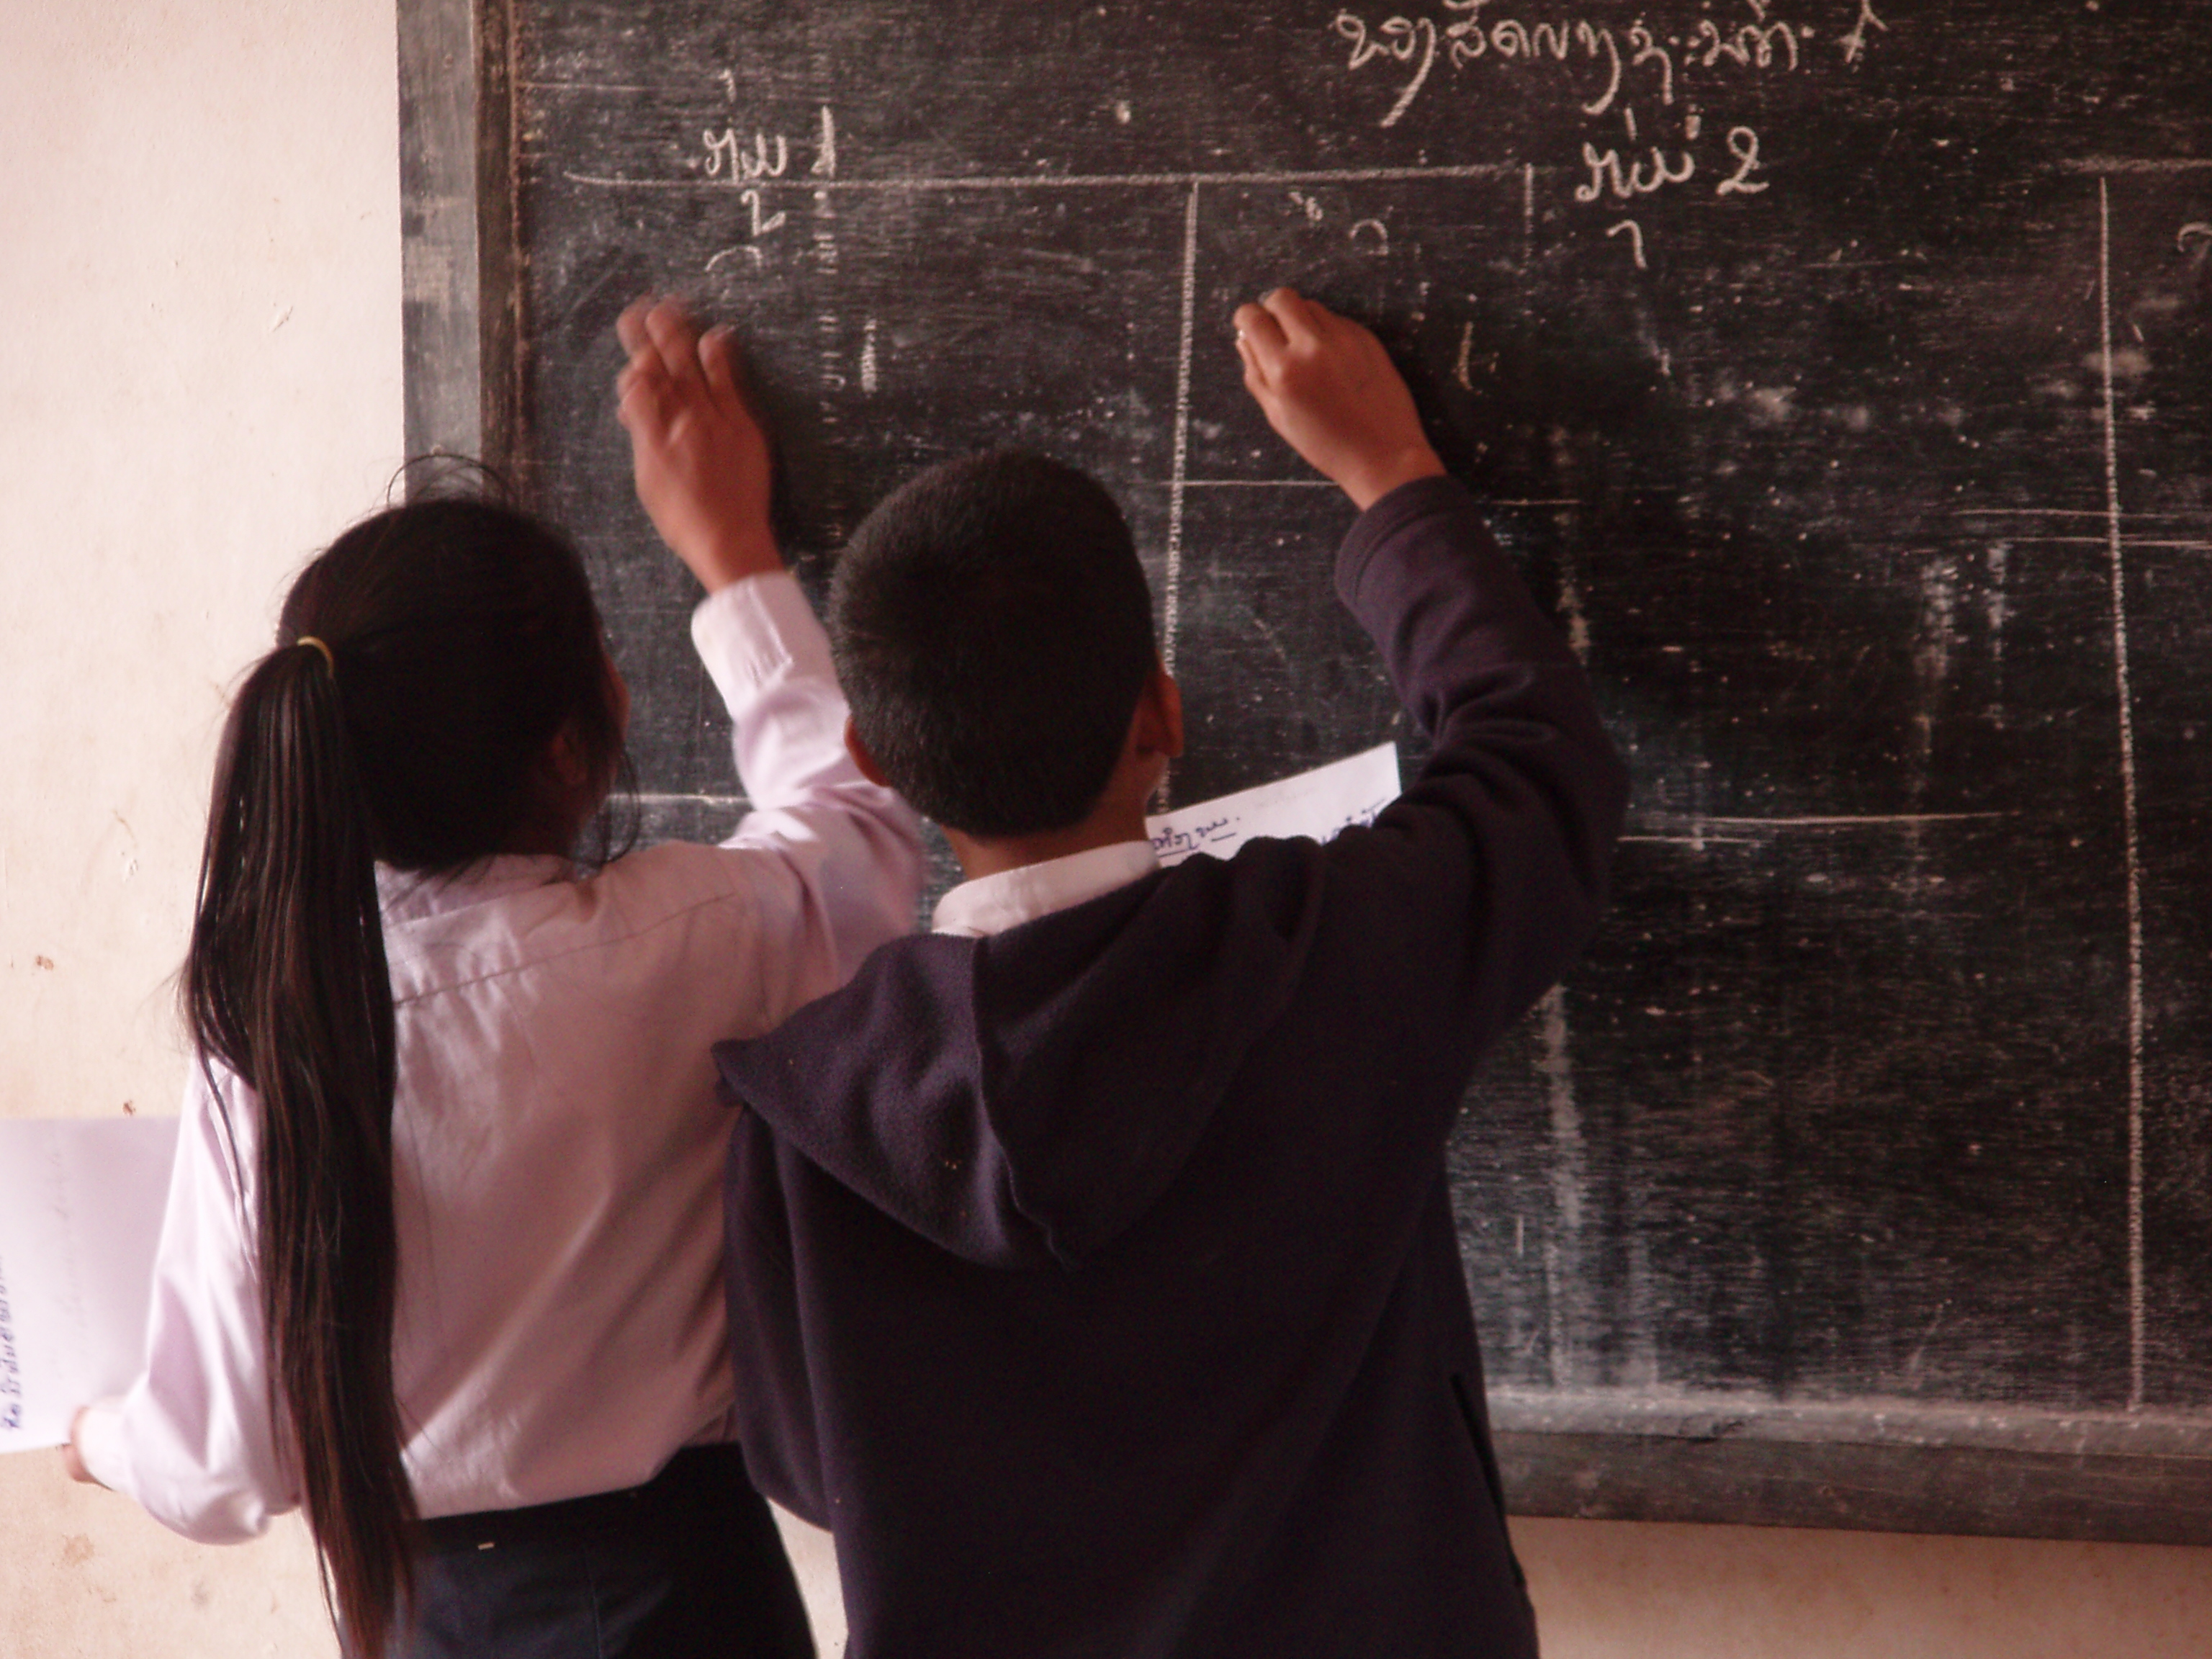
\includegraphics[width=\textwidth]{figures/chalkboard.jpg}
	\end{center}
\end{frame}

\begin{frame}
	\frametitle{Grammar translation}

	\begin{itemize}
		\item El maestro dicta la clase (explica reglas gramaticales) y los alumnos traducen (durante los 50 y los 60)
	\end{itemize}
\end{frame}

\begin{frame}
	\frametitle{Grammar translation}

	\begin{center}
		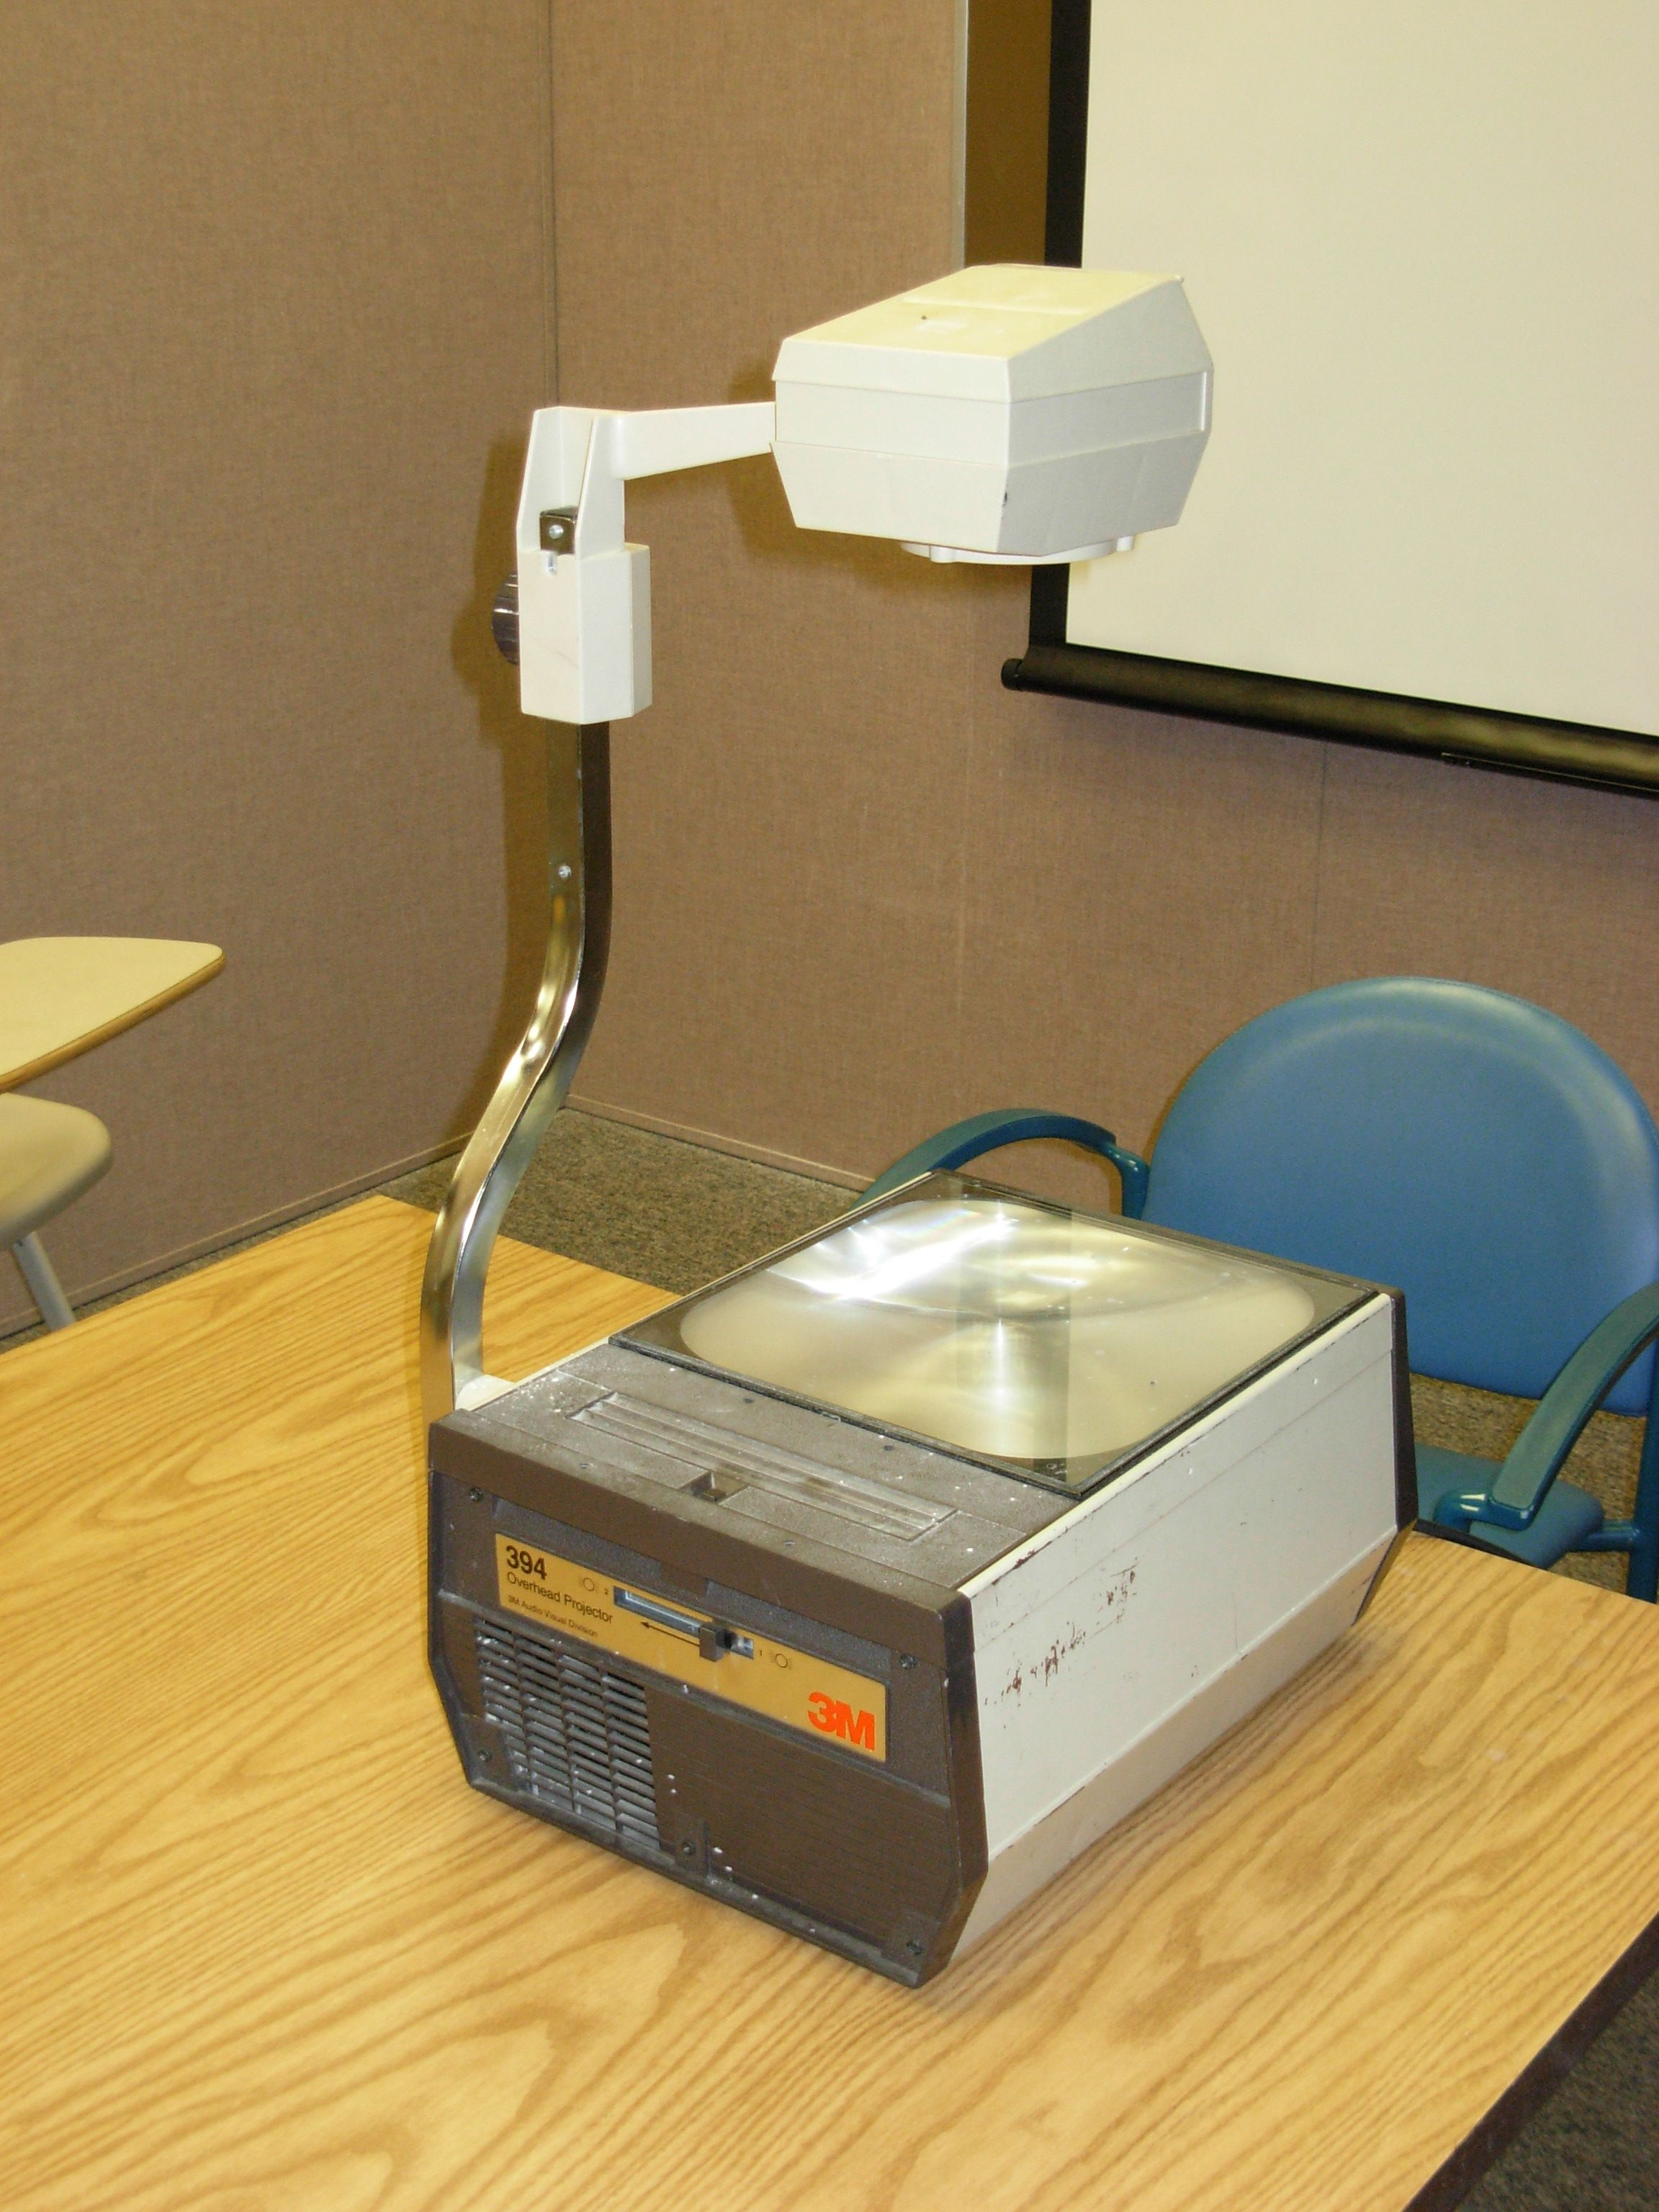
\includegraphics[width=.5\textwidth]{figures/overhead1.JPG}
	\end{center}
\end{frame}

\begin{frame}
	\frametitle{Grammar translation}

	\begin{center}
		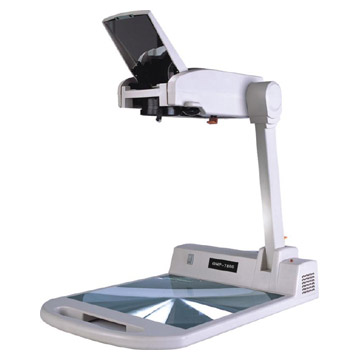
\includegraphics[width=.65\textwidth]{figures/overhead2.JPG}
	\end{center}
\end{frame}

\begin{frame}
	\frametitle{Audiolingüe}

	\begin{itemize}
		\item ¿Qué tecnología se podría usar?
	\end{itemize}
\end{frame}

\begin{frame}
	\frametitle{Audiolingüe}

	\begin{center}
		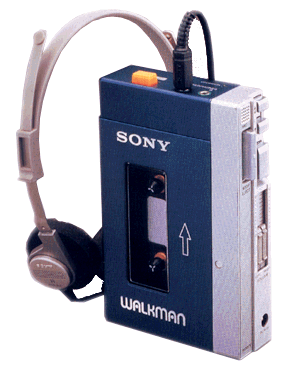
\includegraphics[width=.5\textwidth]{figures/walkman.png}
	\end{center}
\end{frame}

\begin{frame}
	\frametitle{Audiolingüe}

	\begin{itemize}
		\item Se enfatizaba la repitición oral para el aprendizaje
	\end{itemize}
\end{frame}

\begin{frame}
	\frametitle{Audiolingüe}

	\begin{center}
		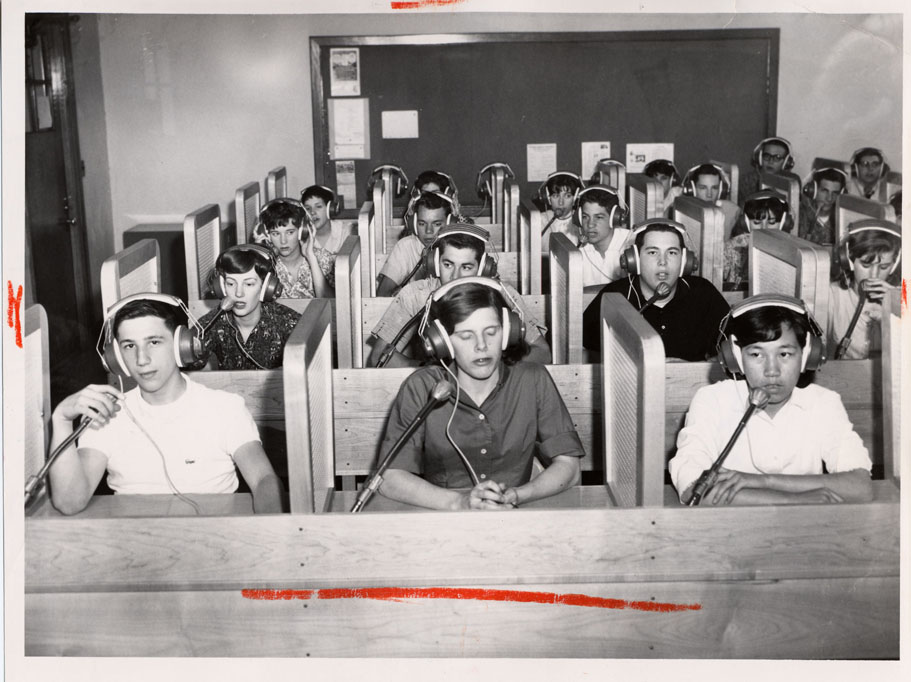
\includegraphics[width=.9\textwidth]{figures/languagelab.jpg}
	\end{center}
\end{frame}

\begin{frame}
	\frametitle{Antes del internet}

	\begin{itemize}
		\item Se pasa por una racha un poco aburrida 
		\item Empieza a haber más software disponible con actividades interactivas 
		\item La interacción sigue siendo poco auténtica/social
	\end{itemize}
	
\end{frame}

\begin{frame}
	\frametitle{Después del internet}

	\begin{itemize}
		\item Webquests  
		\item Email (penpal electrónico)
		\item Multimedia (películas, vídeo, youtube)
		\item videojuegos 
	\end{itemize}
\end{frame}

\begin{frame}
	\frametitle{Después del internet}

	\begin{center}
		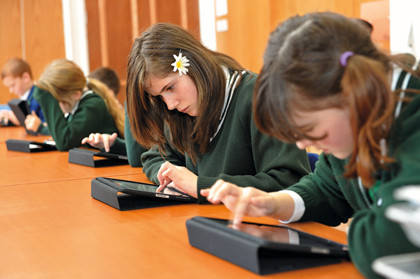
\includegraphics[width=.9\textwidth]{figures/ipad.jpg}
	\end{center}
\end{frame}

\begin{frame}
	\frametitle{Después del internet}

	\begin{center}
		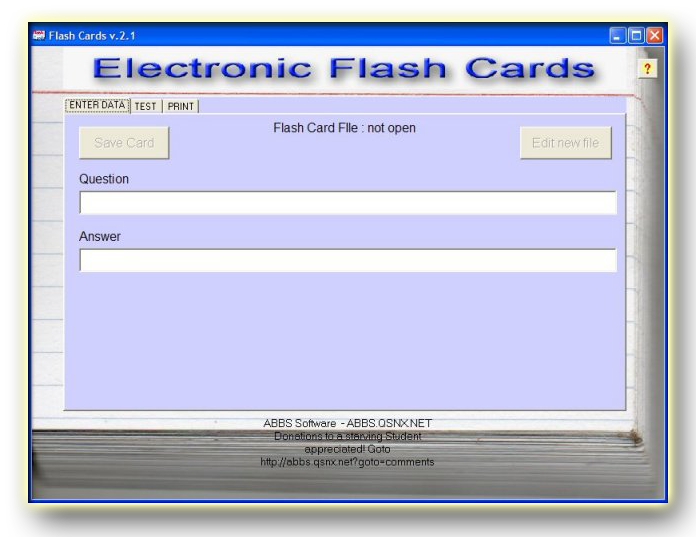
\includegraphics[width=.9\textwidth]{figures/flashcards.png}
	\end{center}
\end{frame}

\begin{frame}
	\frametitle{Después del internet}

	\begin{center}
		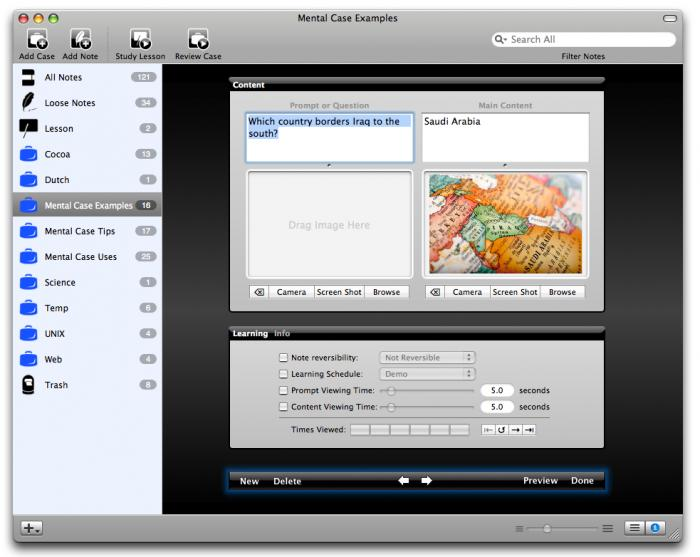
\includegraphics[width=.9\textwidth]{figures/flashcards2.jpg}
	\end{center}
\end{frame}

\begin{frame}
	\frametitle{Después del internet}

	\begin{center}
		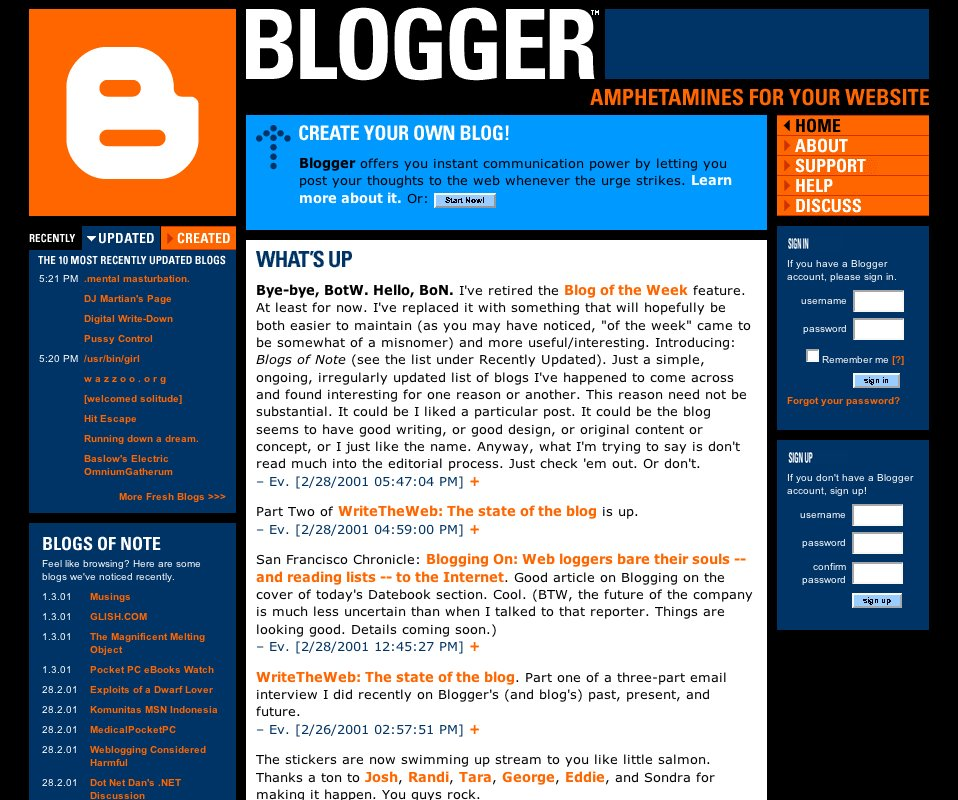
\includegraphics[width=.9\textwidth]{figures/blogger.jpeg}
	\end{center}
\end{frame}

\begin{frame}
	\frametitle{Después del internet}

	\begin{center}
		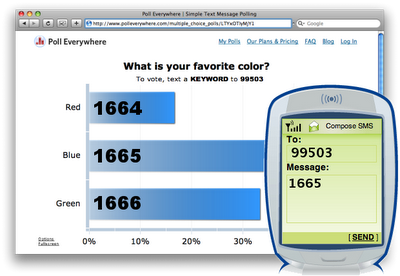
\includegraphics[width=.9\textwidth]{figures/poll_everywhere.png}
	\end{center}
\end{frame}

\begin{frame}
	\frametitle{Después del internet}

	\begin{center}
		
\includegraphics[width=.9\textwidth]{figures/Facebook-Groups.png}
	\end{center}
\end{frame}

\begin{frame}
	\frametitle{Después del internet}

	\begin{center}
		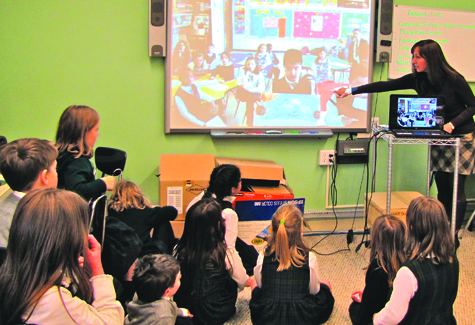
\includegraphics[width=.9\textwidth]{figures/skype.jpg}
	\end{center}
\end{frame}

\begin{frame}
	\frametitle{Después del internet}

	\begin{center}
		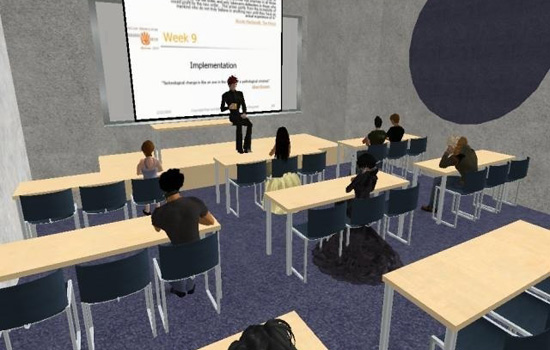
\includegraphics[width=.9\textwidth]{figures/second-life.jpg}
	\end{center}
\end{frame}

\begin{frame}
	\frametitle{Después del internet}

	\begin{center}
		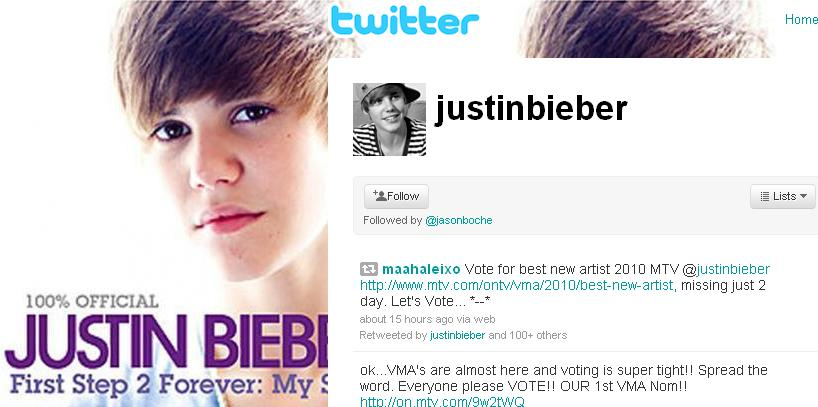
\includegraphics[width=.9\textwidth]{figures/twitter.jpg}
	\end{center}
\end{frame}

\begin{frame}
	\frametitle{Después del internet}

	\begin{center}
		
\includegraphics[width=.9\textwidth]{figures/memes1.jpg}
	\end{center}
\end{frame}

\begin{frame}
	\frametitle{Después del internet}

	\begin{center}
		
\includegraphics[width=.9\textwidth]{figures/memes2.jpg}
	\end{center}
\end{frame}

\begin{frame}
	\frametitle{Después del internet}

	\begin{center}
		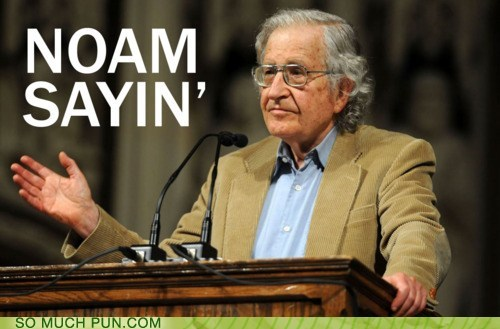
\includegraphics[width=.9\textwidth]{figures/memes3.jpeg}
	\end{center}
\end{frame}





\begin{frame}
	\begin{itemize}
		\item ¿Qué otras tecnologías habéis visto/usado en clase? 
		\item En vuestra experiencia, ¿cómo ayudan/facilitan la enseñanza/el aprendizaje?
	\end{itemize}
\end{frame}

\begin{frame}
	\frametitle{Praat}

	\begin{itemize}
		\item Cada vez más se está utilizando la tecnología para enseñar la pronunciación 
		\item No solamente los segmentos (fonemas), sino también los elementos suprasegmentales (la prosodia)
	\end{itemize}
\end{frame}

\begin{frame}[plain]
	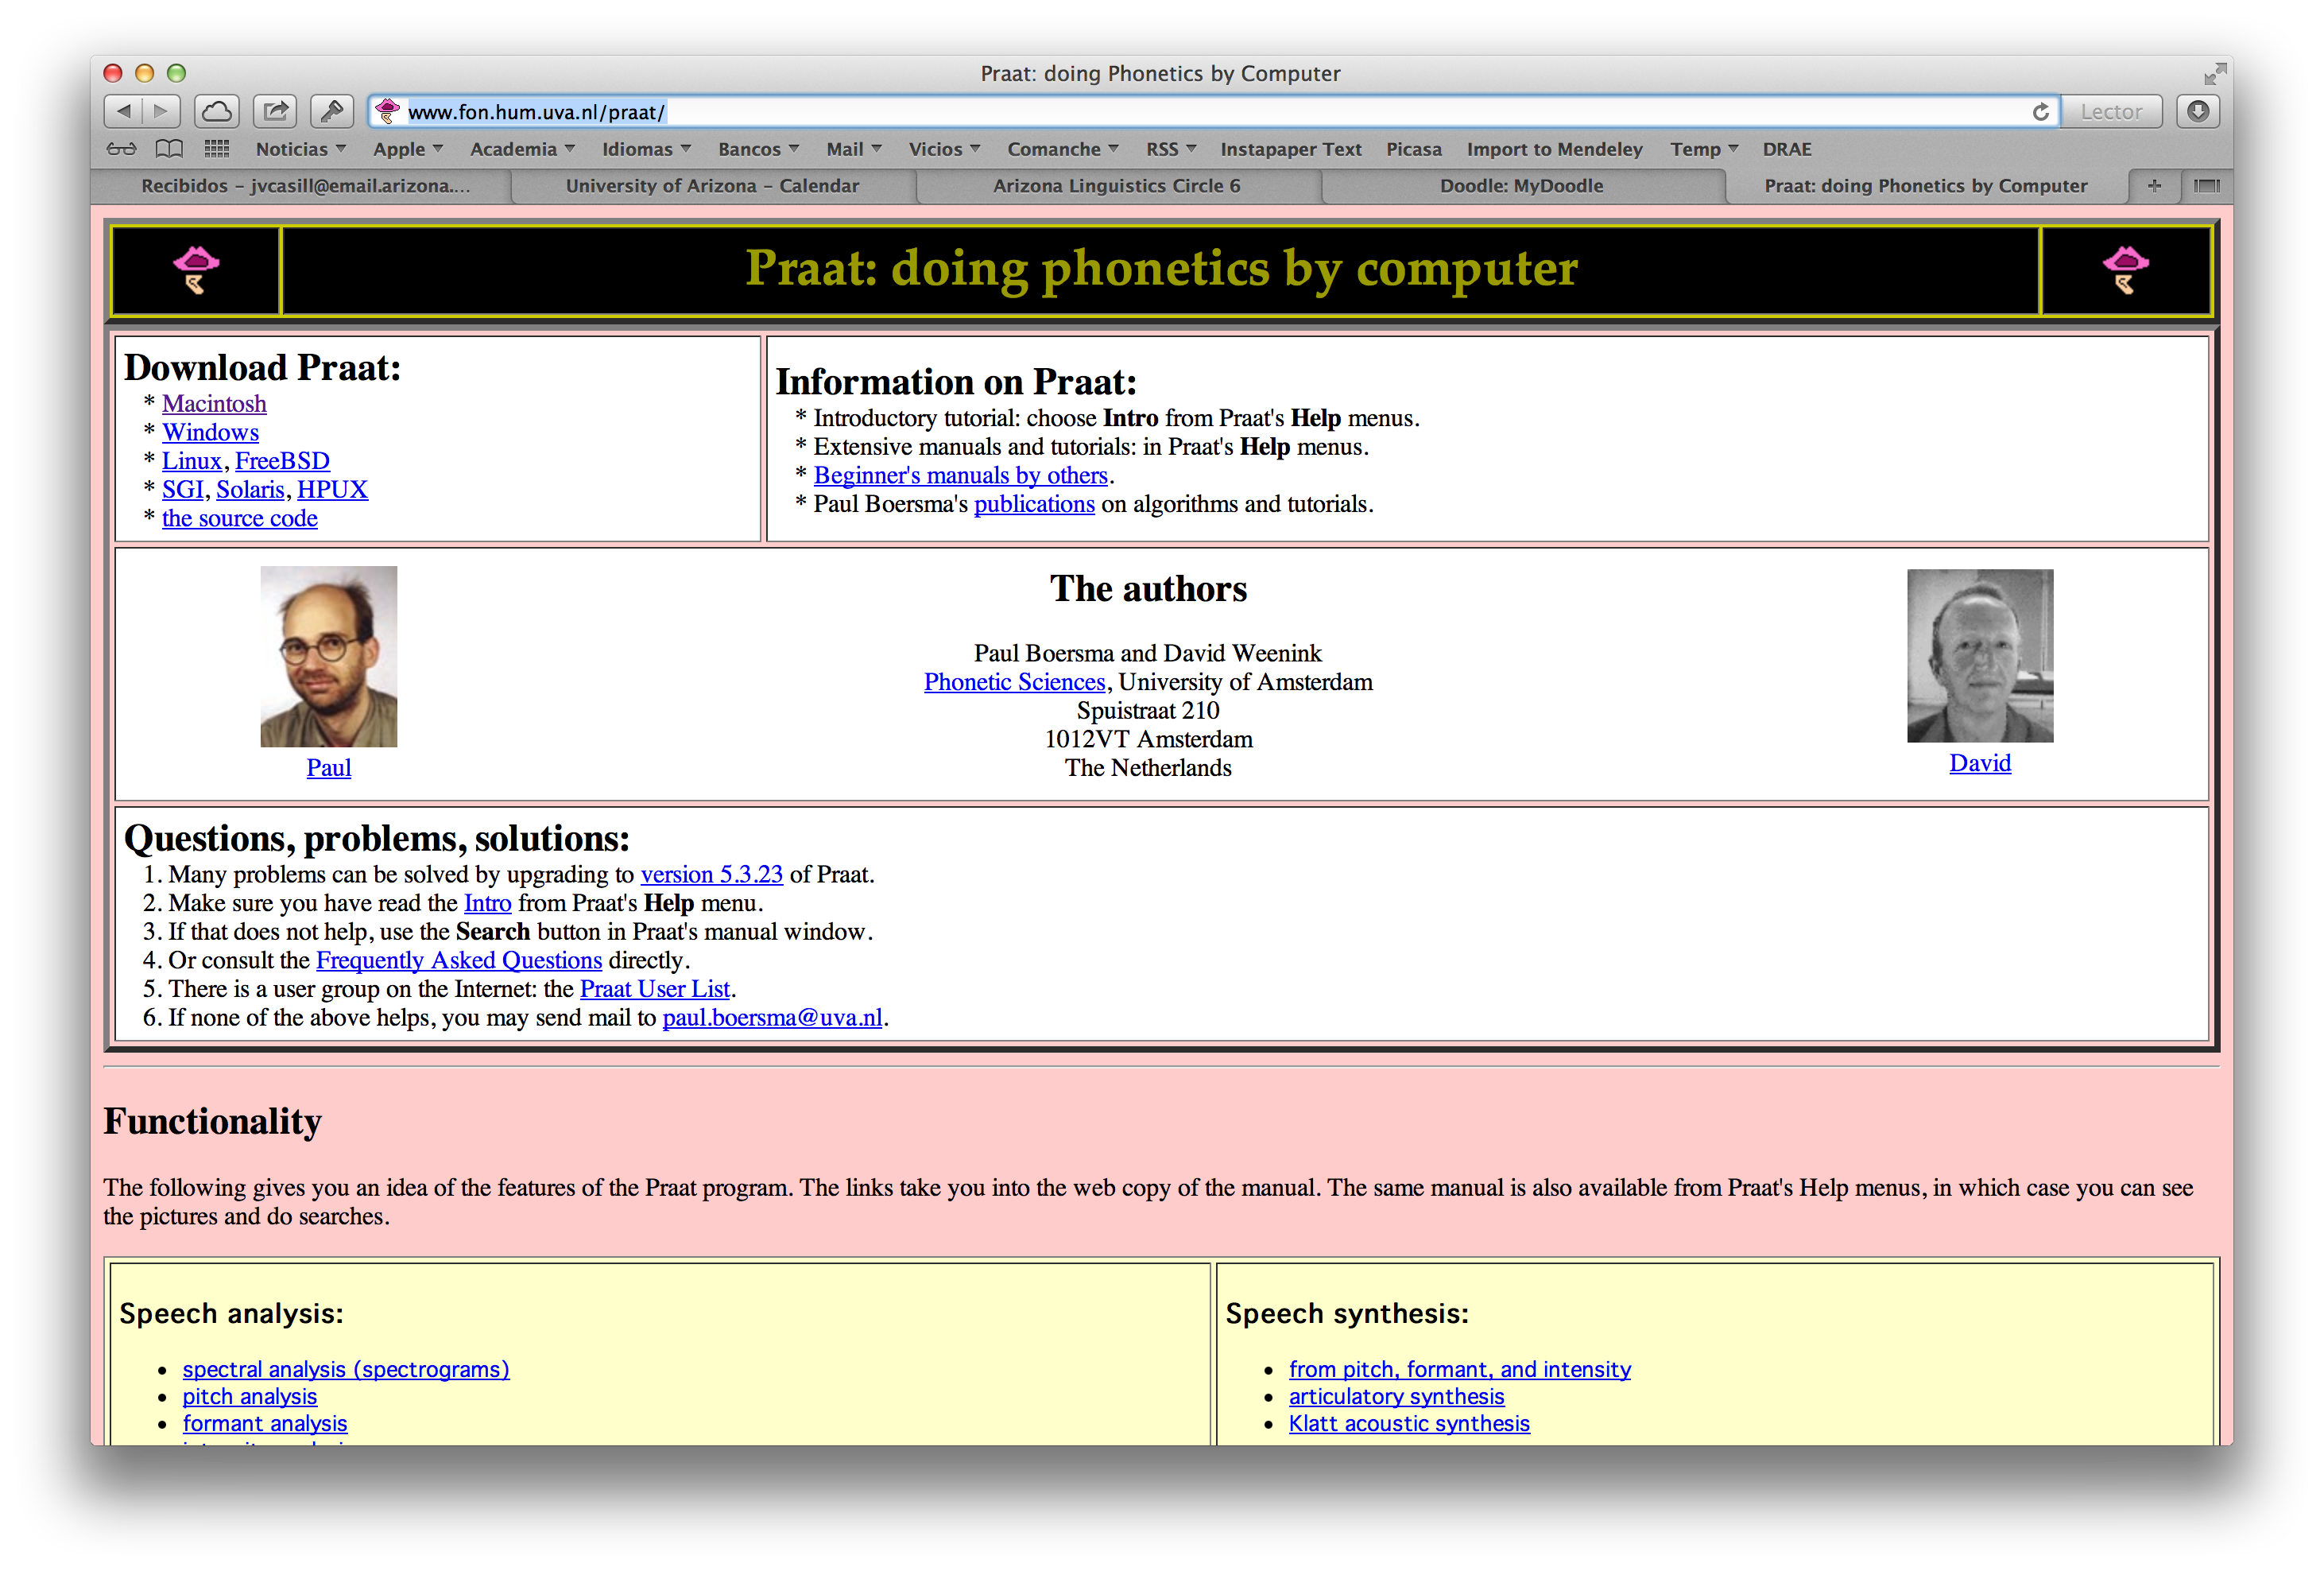
\includegraphics[width=\textwidth]{figures/praat.png}	
\end{frame}

\begin{frame}
	\frametitle{(¿)Llegaron mis amigos(?)}
	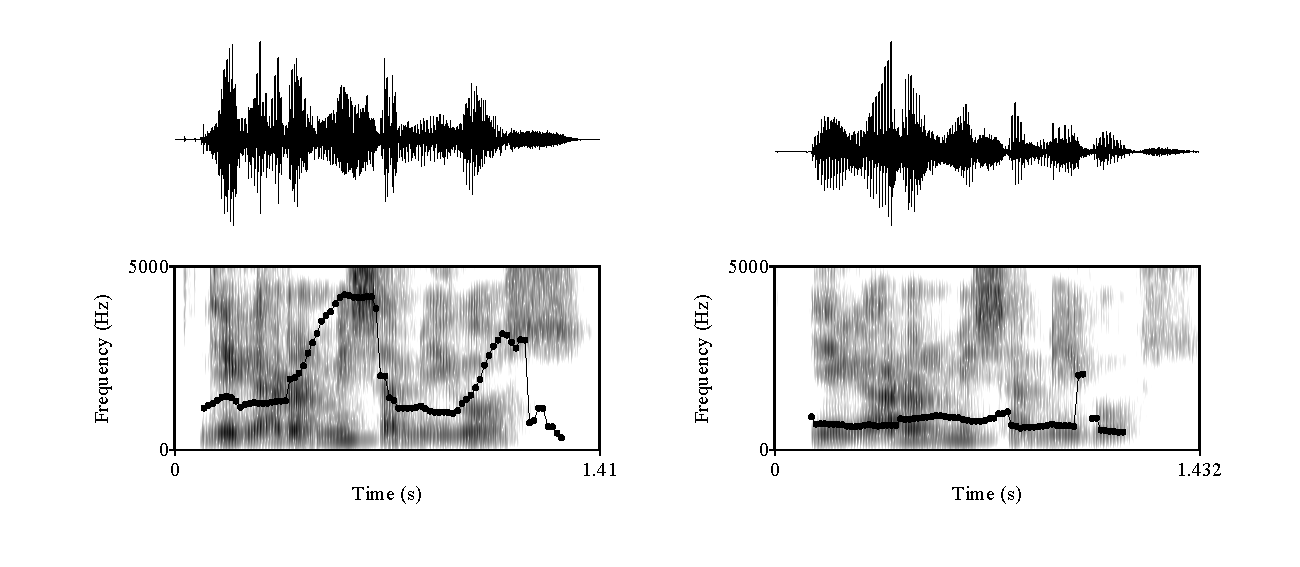
\includegraphics[width=\textwidth]{figures/llegaron.pdf}	
\end{frame}





\begin{frame}
	\frametitle{/t/}

	¿Cuáles son las diferencias entre /t/ del inglés y /t/ del español?

\end{frame}

\begin{frame}
	\frametitle{/t/}

	El sonido /t/ del español difiere del /t/ del inglés en cuanto al punto de articulación y VOT
	\vspace{.2in}

	\begin{itemize}
		\item Punto de articulación: ¿Dónde se produce el contacto al pronunciar /t/?
		\begin{itemize}
			\item /t/ del español es dental 
			\item /t/ del inglés es alveolar
		\end{itemize}
	\end{itemize}
\end{frame}

\begin{frame}
	\frametitle{/t/}

	El sonido /t/ del español difiere del /t/ del inglés en cuanto al punto de articulación y VOT	
	\vspace{.2in}

	\begin{itemize}
		\item VOT (voice-onset time): En las consonantes oclusivas, es la diferencia (en milisegundos) entre la explosión de la consonante y el comienzo de la fonación.
		\begin{itemize}
		 	\item Es el resultado de la coordinación de gestos articulatorios (la explosión y la vibración de las cuerdas vocales)
		 	\item VOT puede ser negativo, 0, o positivo y se usa para contrastar entre sonido sordos/sonoros
		 \end{itemize} 
	\end{itemize}
\end{frame}

\begin{frame}[plain]
	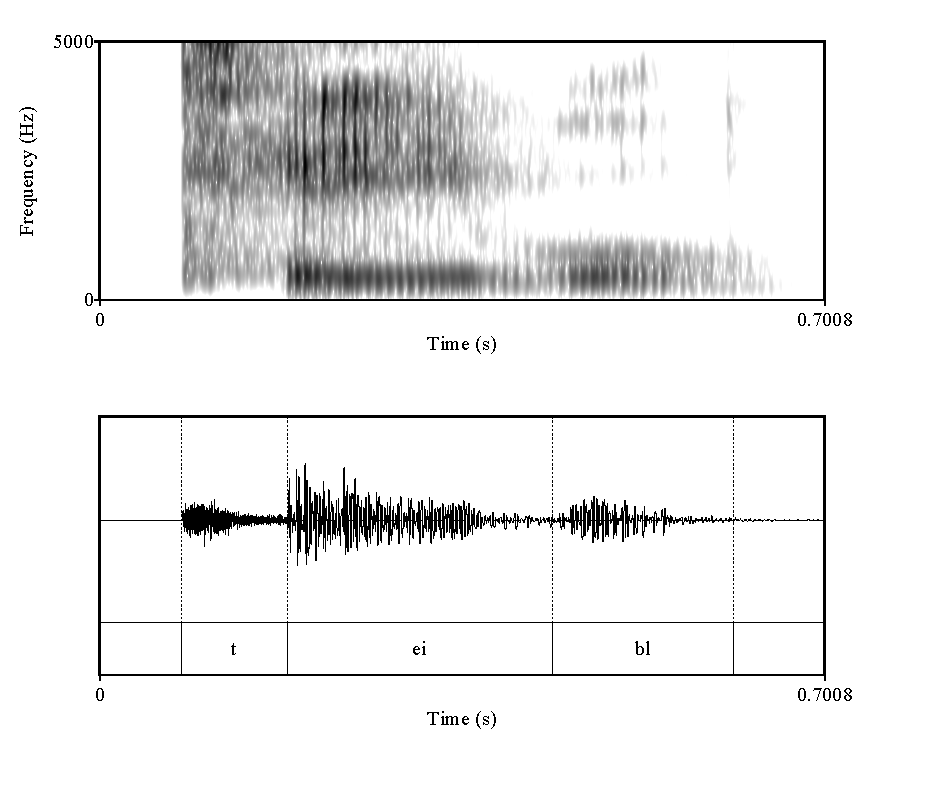
\includegraphics[width=\textwidth]{figures/table.pdf}
\end{frame}

\begin{frame}[plain]
	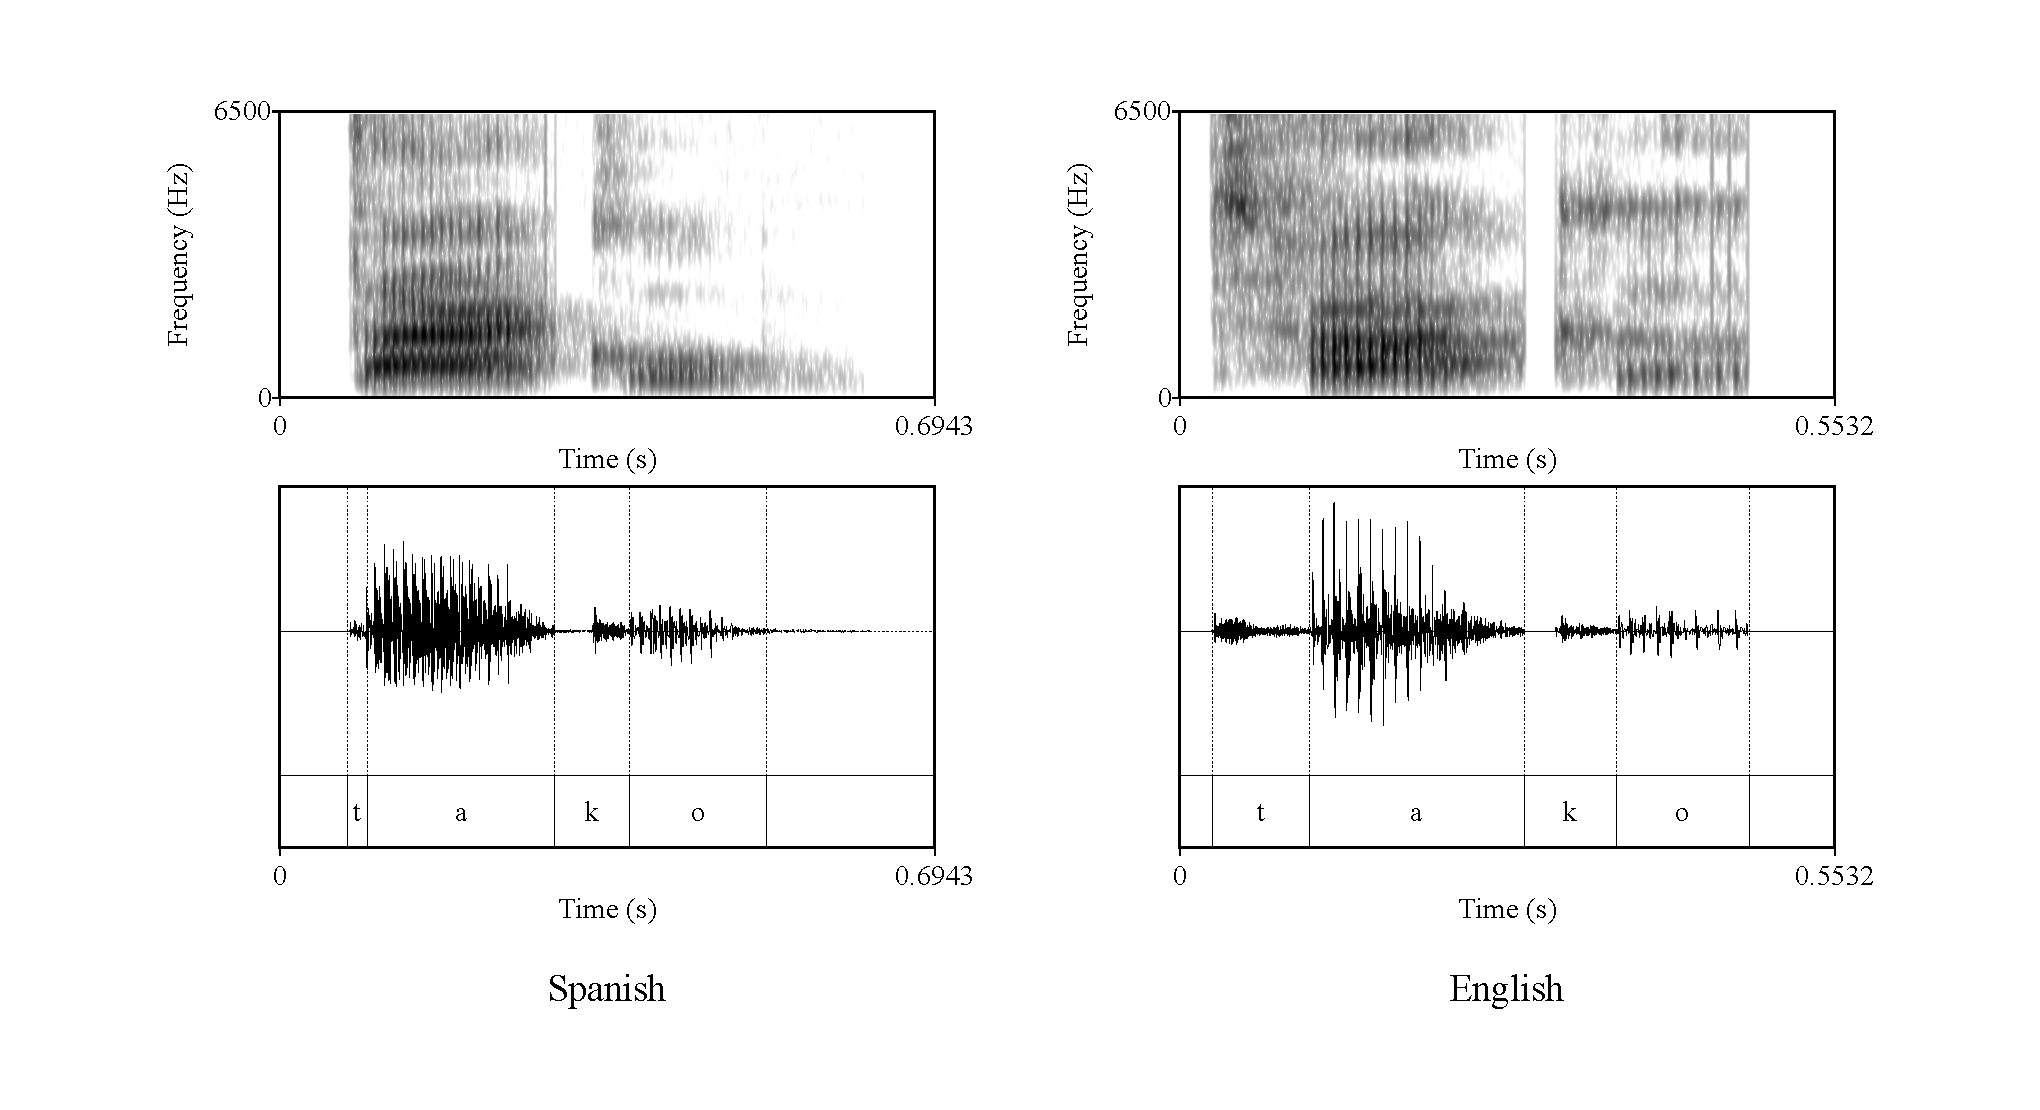
\includegraphics[width=\textwidth]{figures/vot.pdf} \\
	\vspace{.1in}
	\includemedia[
  			addresource=sounds/taco.mp3,
  			flashvars={
    			source=sounds/taco.mp3
   			&autoPlay=true
  			}
		]
		{\fbox{VOT}}{APlayer.swf}
\end{frame}

\begin{frame}
	\frametitle{Resumiendo}
	\framesubtitle{VOT}

	\begin{itemize}
		\item En inglés /t/: 
		\begin{itemize}
			\item se aspira y tiene VOT positivo
			\item el punto de articulación es alveolar
		\end{itemize} 
		\item En español /t/:
		\begin{itemize}
			\item no se aspira y tiene VOT 0 (o muy breve)
			\item el punto de articulación es dental
		\end{itemize} 
		\item Los aprendices del español como L2 tiene que adoptar un PA dental y evitar la aspiración
		\item Los aprendices del inglés como L2 tienen que adoptar un PA alveolar y aspirar
	\end{itemize}
\end{frame}

\begin{frame}
	
	\begin{itemize}
		\item ¿Cómo podemos enseñar esto?
	\end{itemize}
\end{frame}
	


\end{document}